\documentclass[12pt]{report}
\usepackage[utf8]{inputenc}
\usepackage[russian]{babel}
%\usepackage[14pt]{extsizes}
\usepackage{listings}

\usepackage{graphicx}
\graphicspath{{src/}}
\DeclareGraphicsExtensions{.pdf,.png,.jpg}

\usepackage{amsmath,amsfonts,amssymb,amsthm} 

% Для листинга кода:
\lstset{ %
language=c++,                 % выбор языка для подсветки (здесь это С++)
basicstyle=\small\sffamily, % размер и начертание шрифта для подсветки кода
numbers=left,               % где поставить нумерацию строк (слева\справа)
numberstyle=\tiny,           % размер шрифта для номеров строк
stepnumber=1,                   % размер шага между двумя номерами строк
numbersep=5pt,                % как далеко отстоят номера строк от подсвечиваемого кода
showspaces=false,            % показывать или нет пробелы специальными отступами
showstringspaces=false,      % показывать или нет пробелы в строках
showtabs=false,             % показывать или нет табуляцию в строках
frame=single,              % рисовать рамку вокруг кода
tabsize=2,                 % размер табуляции по умолчанию равен 2 пробелам
captionpos=t,              % позиция заголовка вверху [t] или внизу [b] 
breaklines=true,           % автоматически переносить строки (да\нет)
breakatwhitespace=false, % переносить строки только если есть пробел
escapeinside={\#*}{*)}   % если нужно добавить комментарии в коде
}

% Для измененных титулов глав:
\usepackage{titlesec, blindtext, color} % подключаем нужные пакеты
\definecolor{gray75}{gray}{0.75} % определяем цвет
\newcommand{\hsp}{\hspace{20pt}} % длина линии в 20pt
% titleformat определяет стиль
\titleformat{\chapter}[hang]{\Huge\bfseries}{\thechapter\hsp\textcolor{gray75}{|}\hsp}{0pt}{\Huge\bfseries}


% plot
\usepackage{pgfplots}
\usepackage{filecontents}
\usetikzlibrary{datavisualization}
\usetikzlibrary{datavisualization.formats.functions}


\begin{document}
\begin{titlepage}
	\centering
	{\scshape\LARGE МГТУ им. Баумана \par}
	\vspace{3cm}
	{\scshape\Large Лабораторная работа №7\par}
	\vspace{0.5cm}	
	{\scshape\Large По курсу: "Анализ алгоритмов"\par}
	\vspace{1.5cm}
	{\huge\bfseriesПоиск подстроки в строке\par}
	\vspace{2cm}
	\Large Работу выполнила: Оберган Татьяна, ИУ7-55Б\par
	\vspace{0.5cm}
	\LargeПреподаватели:  Волкова Л.Л., Строганов Ю.В.\par

	\vfill
	\large \textit {Москва, 2019} \par
\end{titlepage}

\tableofcontents

\newpage
\chapter*{Введение}
\addcontentsline{toc}{chapter}{Введение}
Цель работы: изучение алгоритмов поиска подстроки в строке.
\newline
Задачи данной лабораторной работы:
\begin{enumerate}
        \item изучить алгоритмы Бойера-Мура и Кнута-Морриса-Пратта;
        \item реализовать эти алгоритмы;
        \item провести тестирование ПО.
\end{enumerate}



\chapter{Аналитическая часть}
В данной части будут рассмотрены алгоритмы поиска подстроки в строке.

\section{Общие сведения об алгоритмах поиска подстроки}
\par
Поиск подстроки в строке — одна из простейших задач поиска информации. Применяется в виде встроенной функции в текстовых редакторах, СУБД, поисковых машинах, языках программирования, программы определения плагиата осуществляют онлайн-проверку, используя алгоритмы поиска подстроки среди большого количества документов, хранящихся в собственной базе\cite{1}.
На сегодняшний день существует огромное разнообразие алгоритмов поиска подстроки. Программисту приходится выбирать подходящий в зависимости от таких факторов: длина строки, в которой происходит поиск, необходимость оптимизации, размер алфавита, возможность проиндексировать текст, требуется ли одновременный поиск нескольких строк.  В данной лабораторной работе будут рассмотремы два алгоритма сравнения с образцом, алгоритм Кнута-Морриса-Пратта и алгоритм Бойера-Мура.

\subsection{Стандартный алгоритм}
Стандартный алгоритм начинает со сравнения первого символа текста с первым символом подстроки. Если они совпадают, то происходит переход ко второму символу текста и подстроки. При совпадении сравниваются следующие символы. Так продолжается до тех пор, пока не окажется, что подстрока целиком совпала с отрезком текста, или пока не встретятся несовпадающие символы. В первом случае задача решена, во втором мы сдвигаем указатель текущего положения в тексте на один символ и заново начинаем сравнение с подстрокой\cite{2}.

\subsection{Алгоритм Бойера-Мура}
Алгоритм Бойера-Мура осуществляет сравнение с образцом справа налево, а не слева направо. Исследуя искомый образец, можно осуществлять более эффективные прыжки в тексте при обнаружении несовпадения. В этом алгоритме кроме таблицы суффиксов применяется таблица стоп-символов. Она заполняется для каждого сивола в алфавите. Для каждогостречающегося в подстроке символа таблица заполняется по принципу максимальной позиции символа в строке, за исключением последнего символа. При определении сдвига при очередном несовпадении строк, выбирается максимальное значение из таблицы суффиксов и стоп-символов\cite{2}.


\subsection{Алгоритм Кнута-Морриса-Пратта}
Алгоритм Кнута-Морриса-Пратта основан на принципе конечного автомата, однако он использует более простой метод обработки неподходящих символов. В этом алгоритме состояния помечаются символами, совпадение с которыми должно в данный момент произойти. Из каждого состояния имеется два перехода: один соответствует успешному сравнению, другой - несовпадению. Успешное сравнение переводит нас в следующий узел автомата, а в случае несовпадения мы попадаем в предыдущий узел, отвечающий образцу. 
В программной реализации этого алгоритма применяется массив сдвигов, который создается для каждой подстроки, которая ищется в тексте. Для каждого символа из подстроки рассчитывается значение, равное максимальной длине совпадающего префикса и суффикса отсительно конкретного элемента подстроки. Создание этого массива позволяет при несовпадении строки сдвигать ее на расстояние, большее, чем 1 (в отличие от стандартного алгоритма).

\section*{Вывод}
\addcontentsline{toc}{section}{Вывод}
В данном разделе были рассмотрены основные алгоритмы поиска подстроки в строке.



\chapter{Конструкторская часть}
В данном разделе будут рассмотрены основные требования к программе и пошлаговая работа алгоритмов.

\section{Требования к программе}

\textbf{Требования к вводу:}
Длина подстроки должна быть больше, чем длина строки.
\newline
\textbf{Требования к программе:}
\begin{itemize}
\item каждая из функций должна выдавать первый индекс вхождения подстроки в строку;
\item если строка не содержит подстроку, то функция выдает -1.
\end{itemize}

\section{Пример работы алгоритмов}
В таблице 1 и таблице 2 буде рассмотрена пошаговая работа алгоритмов Кнута-Морриса-Пратта и Бойера-Мура на значениях строки s и подстроки sub.  

string s = "ababacabaa";  
string sub = "abaa";   

\subsection{Алгоритм Кнута-Морриса-Пратта}
Для алгоритма Кнута-Морриса-Пратта вычисленный массив префиксов для заданой  подстроки sub имеет значение:
prefix = [0, 0, 1, 1]

Таблица 1 отображает пошаговую работу алгоритма Кнута-Морриса-Пратта при данном массиве префиксов.
 
\begin{center}
Таблица 1. Пошаговая работа алгоритма Кнута-Морриса-Пратта.\\

\begin{tabular}{| c | c | c | c | c | c | c | c | c | c | }
	\hline
	a&b&a&b&a&c&a&b&a&a \\
	\hline
	\hline
	a&b&a&\textcolor{red}{a}&&&&&&\\
	\hline
	&&a&b&a&\textcolor{red}{a}&&&&\\
	\hline
	&&&&a&\textcolor{red}{b}&a&a&&\\
	\hline
	&&&&&\textcolor{red}{a}&b&a&a&\\
	\hline
	&&&&&&a&b&a&\textcolor{green}{a}\\
	\hline

	
\end{tabular}
\end{center}

\subsection{Алгоритм Бойера-Мура}
Для алгоритма Бойера-Мура вычисленный массив суффиксов для заданой  подстроки sub имеет значение:
suffix = [2, 5, 5, 6].
Переходы алфавита для подстроки sub:
letters = ['a' = 0, 'b' = 2]   
Если буквы нет в letters, будет считаться, что переход равен длиние sub.

\begin{center}
Таблица 2. Пошаговая работа алгоритма Бойера-Мура.\\

\begin{tabular}{| c | c | c | c | c | c | c | c | c | c | }
	\hline
	a&b&a&b&a&c&a&b&a&a \\
	\hline
	\hline
	a&b&a&\textcolor{red}{a}&&&&&&\\
	\hline
	&&a&b&a&\textcolor{red}{a}&&&&\\
	\hline
	&&&&&&\textcolor{green}{a}&b&a&a\\
	\hline

	
\end{tabular}
\end{center}


\section*{Вывод}
\addcontentsline{toc}{section}{Вывод}
В данном разделе были рассмотрены основные требования к программе, разобрана работа алгоритмов на конкретной строке и подстроке.

 

\chapter{Технологическая часть}
Замеры времени были произведены на: Intel(R) Core(TM) i5-8300H, 4 ядра, 8 логических процессоров.

\section{Выбор ЯП}
В качестве языка программирования был выбран C\# \cite{Microsoft}. Средой разработки Visual Studio. 
Время работы алгоритмов было замерено с помощью класса Stopwatch. Тестирование было реализовано
с помощью стандартного шаблона модульных тестов\cite{UnitTests}.

\section{Сведения о модулях программы}
Программа состоит из:
\begin{itemize}
	\item Program.cs - главный файл программы, в котором располагается точка входа в программу
	\item StrMatching.cs - функции поиска подстроки
	%\item lab_7_SubstrTest - проект для тестировании программы
\end{itemize}


\section{Листинг кода алгоритмов}
В этой части будут рассмотрены листинги кода (листинг 3.1 - 3.5) реализованых алгоритмов.
\begin{lstlisting}[label=some-code,caption=Стандартная функция]
public static int Standard(string str, string substr)
        {
            for (int i = 0; i <= str.Length - substr.Length; i++)
            {
                bool correct = true; 
                for (int j = 0; j < substr.Length && correct; j++)
                {
                    if (str[i + j] != substr[j])
                        correct = false;
                }
                if (correct)
                    return i;
            }
            return -1;
        }
\end{lstlisting}

\begin{lstlisting}[label=some-code,caption=Алгоритм KMP]
public static int KMP(string str, string substr)
        {
            int[] prefix = PrefixFunction(substr);
            int last_prefix = 0;
            for (int i = 0; i < str.Length; i++)
            {
                while (last_prefix > 0 && substr[last_prefix] != str[i])
                    last_prefix = prefix[last_prefix - 1];

                if (substr[last_prefix] == str[i])
                    last_prefix++;

                if (last_prefix == substr.Length)
                {
                    return i + 1 - substr.Length;
                }
            }
            return -1;
        }
\end{lstlisting}

\begin{lstlisting}[label=some-code,caption=Функция нахождения массива сдвигов]
static int[] PrefixFunction(string substr)
        {
            int[] prefix = new int[substr.Length];

            int lastPrefix = prefix[0] = 0;
            for (int i = 1; i < substr.Length; i++)
            {
                while (lastPrefix > 0 && substr[lastPrefix] != substr[i])
                    lastPrefix = prefix[lastPrefix - 1];

                if (substr[lastPrefix] == substr[i])
                    lastPrefix++;

                prefix[i] = lastPrefix;
            }
            return prefix;
        }
\end{lstlisting}


\begin{lstlisting}[label=some-code,caption= Алгоритм Бойера-Мура]
public static int BM(string str, string substr)
        {
            if (substr.Length == 0)
                return -1;
            
            Dictionary<char, int> letters = new Dictionary<char, int>();
            for (int i = 0; i < substr.Length; i++)
                if (letters.ContainsKey(substr[i]))
                    letters[substr[i]] = substr.Length - 1 - i;
                else
                    letters.Add(substr[i], substr.Length - 1 - i);

            int[] suffix = GetSuffix(substr);

            for (int i = substr.Length - 1; i < str.Length;)
            {
                int j = substr.Length - 1;
                while (substr[j] == str[i])
                {
                    if (j == 0)
                        return i;
                    i--;
                    j--;
                }
                var a = letters.ContainsKey(str[i]) ? letters[str[i]] : substr.Length;
                var b = suffix[substr.Length - 1 - j];
                i += Math.Max(a, b);
            }
            return -1;
        }
\end{lstlisting}

\begin{lstlisting}[label=some-code,caption=Функция вычисления сдвигов суффиксов]
        static int[] GetSuffix(string substr)
        {
            int[] table = new int[substr.Length];
            int lastPrefixPosition = substr.Length;

            for (int i = substr.Length - 1; i >= 0; i--)
            {
                if (IsPrefix(substr, i + 1))
                    lastPrefixPosition = i + 1;
                table[substr.Length - 1 - i] = lastPrefixPosition - i + substr.Length - 1;
            }

            for (int i = 0; i < substr.Length - 1; i++)
            {
                int slen = SuffixLength(substr, i);
                table[slen] = substr.Length - 1 - i + slen;
            }

            return table;
        }
\end{lstlisting}

\section{Тестирование программы}
 В этой части будет рассмотрен листинг функций тестирования алгоритмов (листинг 3.6 -3.7). 
\begin{lstlisting}[label=some-code,caption=Тестирование функции случайными значениями]
[TestMethod]
        public void TestStandardRandom()
        {
            for (int i = 0; i < N; i++)
            {
                string s = rand.Next(1000, 9999999).ToString();
                string sub = rand.Next(100, 999).ToString();

                int iCorrect = s.IndexOf(sub);
                int res = lab_7_Substr.StrMatching.Standard(s, sub);
                Assert.AreEqual(iCorrect, res, "str: " + s + " sub: " + sub);
            }
        }
\end{lstlisting}

\begin{lstlisting}[label=some-code,caption=Тестирование функции случайными значениями одной длины]
[TestMethod]
        public void TestStandardSameLength()
        {
            for (int i = 0; i < N; i++)
            {
                string s = rand.Next(100, 999).ToString();
                string sub = rand.Next(100, 999).ToString();

                int iCorrect = s.IndexOf(sub);
                int res = lab_7_Substr.StrMatching.Standard(s, sub);
                Assert.AreEqual(iCorrect, res, "str: " + s + " sub: " + sub);
            }
        }
\end{lstlisting}


На рис. 3.1 предоставлен скриншот результатов работы тестов, на котором видно, что алгоритмы работают правильно.

\begin{figure}[h]
	\center{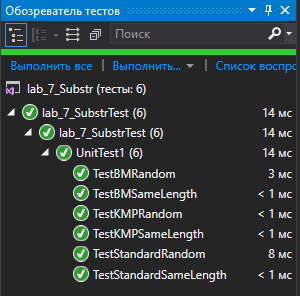
\includegraphics[scale = 1]{src/Testing.png}}
	\caption{Результат работы тестов}
	\label{fig:v_st}
\end{figure}


\section*{Вывод}
\addcontentsline{toc}{section}{Вывод}
В данном разделе были рассмотрены основные сведения о модулях программы, листинг кода алгоритмов и тестов, результаты тестирования,
которое показало,  что алгоритмы реализованы корректно.


\chapter{Исследовательская часть}
В данном разделе будет проведен временной анализ работы алгоритмов.

\section{Сравнительный анализ на основе замеров времени}
Был проведен замер времени работы алгоритмов при разных размерах строки и фиксированом размере подстроки.

\begin{tikzpicture}
\begin{axis}[
    	axis lines = left,
    	xlabel = {Длина},
    	ylabel = {Время (тики)},
	legend pos=south east,
	ymajorgrids=true
]


\addplot[color=blue] table[x index=0, y index= 1] {src/Standard.txt}; 
\addlegendentry{Стандартный}

\addplot[color=orange] table[x index=0, y index= 1] {src/BM.txt}; 
\addlegendentry{BM}

\addplot[color=red] table[x index=0, y index= 1] {src/KMP.txt}; 
\addlegendentry{KMP}

\end{axis}
\end{tikzpicture}
\begin{center}
Pис. 4.1: Сравнение времени работы алгоритмов при увеличении длины строки. Длина подстроки 3
\end{center}

На рисунке 4.1 видно, что моя реализация алгоритма Бойера-Мура проигрывает стандартному и Кнута-Морриса-Пратта.
Это происходит потому что в моей реализации Бойера-Мура используется словарь и в каждом цикле происходит проверка наличия ключа в словаре, из-за чего
и замедляется работа. 

\section*{Вывод}
\addcontentsline{toc}{section}{Вывод}
Сравнительный анализ по времени показал, что внедрение словаря сильно замедляет алгоритм Бойера-Мура.



\chapter*{Заключение}
\addcontentsline{toc}{chapter}{Заключение}
В ходе лабораторной работы я изучила возможности применения и реализовала алгоритмы поиска подстроки в строке. 

Было проведено тестирование, показавшее, что алгоритмы реализованы правильно.

Временной анализ показал, что неэффективно использовать структуру словаря для реализации алгоритма Бойера-Мура.


\addcontentsline{toc}{chapter}{Список литературы}
 \begin{thebibliography}{3}
\bibitem{1} Окулов С. М. Алгоритмы обработки строк. — М.: Бином, 2013. — 255 с.
\bibitem{2} Дж. Макконнелл. Анализ лгоритмов. Активный обучающий подход

\bibitem{Microsoft}
Руководство по языку C\#[Электронный ресурс], - режим доступа: https://docs.microsoft.com/ru-ru/dotnet/csharp/
\bibitem{UnitTests}
Основные сведения о модульных тестах [Электронный ресурс], - режим доступа: https://docs.microsoft.com/ru-ru/visualstudio/test/unit-test-basics?view=vs-2019
\end{thebibliography}


\end{document}